\section{提案} \label{sec:proposal}

\subsection{概要}

本論では,Unikernel の \rr を効率的に行う \emph{VampOS}を紹介する.
VampOS の設計目標は以下のとおりです.

\begin{itemize}
    \item \textbf{Unikernel レイヤのみの Reboot-based Recovery.}{\sysname は,従来の Unikernel の再起動とは異なり,アプリケーションのメモリの内容を保持したまま Unikernel のメモリを若返らせる.アプリケーションは,私たちの Unikernel の再起動に渡って,継続して動作することができる.}
    \item \textbf{特定の Unikernel の構成に依存しない.}{特定の Unikernel のコンポーネントを対象とする \rr のメカニズムは,Unikernel の構成がアプリケーションごとに異なるため,合理的ではない.私たちのアプローチは,どのような Unikernel のコンポーネントにも適用できる.}
    \item \textbf{ダウンタイムをできるだけ短くする.}{\sysname は Unikernel の再起動によるアプリケーションのダウンタイムをできる限り短縮する.}
\end{itemize}

\begin{figure}[t]
    \begin{center}
      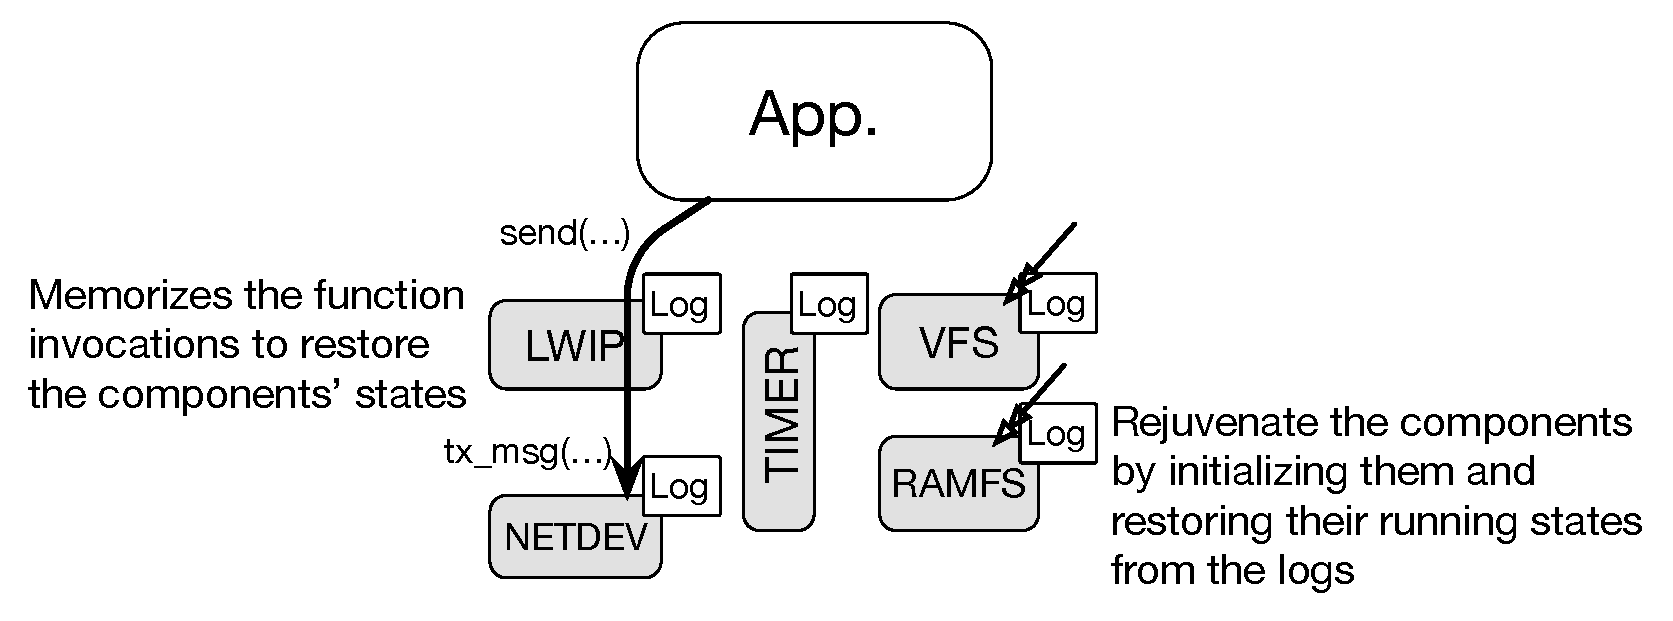
\includegraphics[scale=0.3]{./img/vampos.eps}
      \caption{{\sysname} の概要} 
      \label{fig:overview}
    \end{center}
\end{figure}

これらの目標を達成するために,\sysname は Unikernel のカスタマイズ性を利用している.
Unikernel は多数のコンポーネントを提供し,
コンポーネント間のインタフェースが明確に定義されているため,
アプリケーションの動作に必要なコンポーネントのみを選択することができる.
\sysname の概要を図\ref{fig:overview}に示す.
\sysname はコンポーネント単位での Unikernel の若返りを可能にし,
リンクしたアプリケーションを継続して実行できるように,
若返りしたコンポーネントの動作状態を復元する.
具体的には,\sysname は,公開されているコンポーネントインタフェースをフックすることにより,コンポーネント間のインタラクションを記録し,
ログを再生することで,状態を持つコンポーネントの動作状態を復元する.
例えば,ファイルシステムの若返りにおいては,\sysname は,
他のコンポーネントの動作状態の変更しないように,
そのコンポーネントのみを再起動し,若返りしたコンポーネント内部でログを再生する.

また,\sysname では,\rr による Unikernel の若返りの効果を最大化するために,
コンポーネント間のエラー伝搬を防止する.
コンポーネントのフォルトが別のコンポーネントへと伝搬することで,
複数のコンポーネントでフォルト発生するが,
コンポーネント単位での再起動では,
一度に一つのコンポーネントのエラー状態しか解消することができない.
そのような場合,
Unikernel 全体を安定化させるためには,
フォルト状態にあるコンポーネントすべての若返りが必要になってしまう.

% The window-based interaction between components requires effi-
% cient fine-grained control over page permissions. We propose to use
% Intel’s Memory Protection Keys (MPK) [25], an ISA extension that
% manages access permissions on groups of pages. It was first intro-
% duced in Intel’s Skylake architecture, and it is similar to protection
% keys in Itanium [24] and access identifiers in PA-RISC [23].


\sysname の目標は,\rr の効果を得ることであり,通常の再起動との完全な互換を目指しているものではない.
Unikernel を若返りのために,Unikernel がリンクしたアプリケーションの再起動の代わりに \sysname の再起動することができる.
\sysname のメカニズムは,
通常の再起動によるソフトウェアアップデートや再構成のような他の目的に適用するものではなく,
そのような目的のためには,通常の再起動が使われる.

\sysname の設計は以下の技術的な課題を提示する.
どのように,Unikernel をコンポーネント単位で若返らせるのか?
どのように,対象のコンポーネントのみを復元するのか?
どのように,若返りしたコンポーネントの状態を効率良く復元するのか?
次の章では,これらの課題に対する解決策を述べる.
以下の議論は Unikraft~\cite{KuenzerEtAl-Unikraft} 上のプロトタイプの開発に基づくものであるが,
IncludeOS~\cite{BratterudEtAl-IncludeOS} のような他の Unikernel にも十分に適用できる一般性を持つであろう.
